% Dokumentation
\section{Dokumentation}

Das Frontend von \kort{} ist durchgängig mit der Sencha-eigenen JavaScript-Dokumentationssprache \brand{JSDuck}\footnote{\url{https://github.com/senchalabs/jsduck}} dokumentiert.
Die Dokumentation findet sich unter: \url{http://kort.herokuapp.com/docs/Kort}.

\begin{figure}[H]
	\centering
	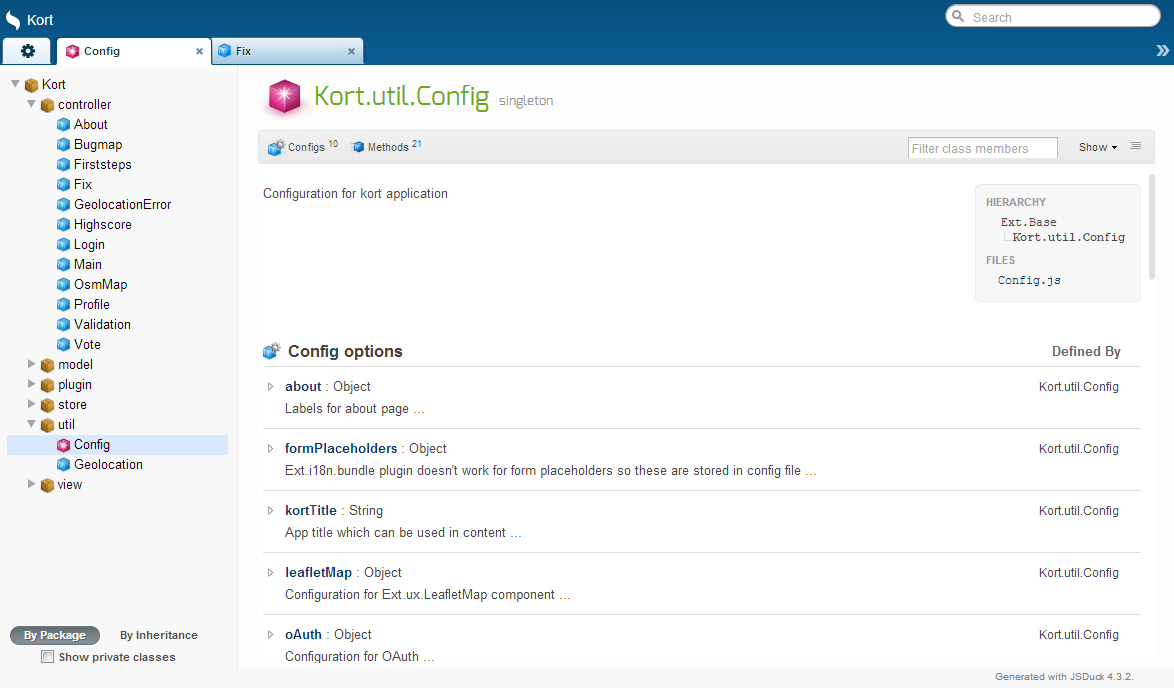
\includegraphics[width=\textwidth]{images/implementation/frontend/kort-documentation}
	\caption{Frontend Dokumentation mit JSDuck}
	\label{image-kort-documentation}
\end{figure}